\chapter{Planteamiento e introducción teórica}

El siguiente diagrame en bloques sintetiza las distintas etapas de la fuente, Desde la entrada de
$220V$ en CA hasta llegar a la tension en CC a la salida.

\begin{figure}[h]
  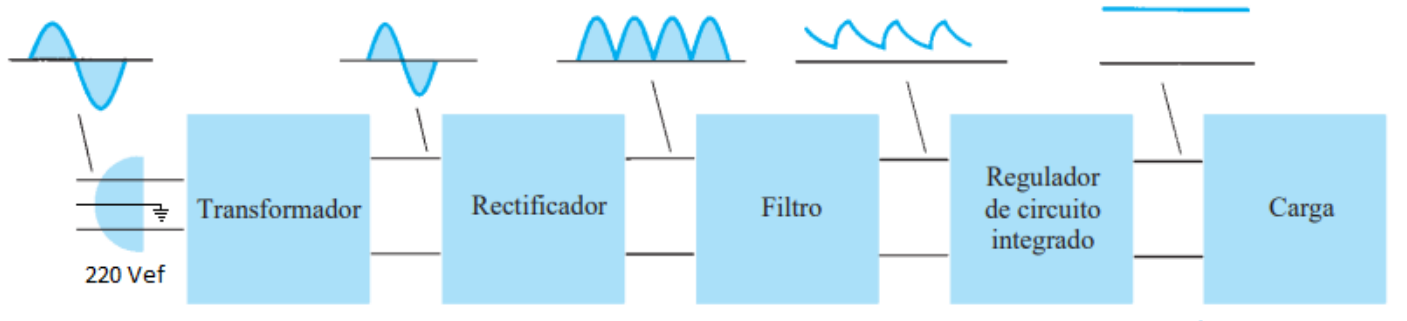
\includegraphics[width=0.95\textwidth]{images/diagramaBloques.png}
  \caption{Diagrama en bloques}
\end{figure}

A contunuación, se explica detaladamente cada uno de estos bloques.

\section{Transformador}
\label{sec:transformador}

El transformador tiene dos funciones:
\begin{itemize}
  \item Aislar galvánicamente el circuito de la red electrica.
  \item Reducir la tension de entrada al valor necesario para la fuente.
\end{itemize}

\begin{circuitikz}
  \draw (0,0) to [sV] ++(0,2) -- ++(1,0)
  node[transformer core, circuitikz/inductors/coils=6,
  anchor=A1](T){};
  \draw (T.A2) -| (0,0);
  \draw (T-L2.midtap) to[short, *-] (T.B1 |- T-L2.midtap);
  \draw (T.B2) to[short, -o] ++(1.2,0);
  \draw (T.B1) ++(0.6,-0.55) node[spdt, rotate=180](SW){} ;
  \draw (T.B1) -| (SW.out 2);
  \draw (T-L2.midtap) -| (SW.out 1);
  \node [ocirc] at (SW.in){};
\end{circuitikz}

En nuestro caso particular, utilizaremos un transformador con punto medio, que a travez de una llave selectora
nos permitirá elegir entre una tension de entrada a nuestra fuente de $12$ o $24\V$.

\hspace{5mm}

\begin{figure}[h]
  \centering
  \begin{circuitikz}
    \draw (0,2) to[short, o-] ++(1,0)
    node[transformer core, circuitikz/inductors/coils=6,
    anchor=A1](T){};
    \draw (T.A2) to[short, -o] ++(-1,0);
    \node at ($($(T.A1)!0.5!(T.A2)$) +(-1,0)$) []{$220\V$};

    \draw (T-L2.midtap) to[short, *-] (T.B1 |- T-L2.midtap);
    \draw (T.B2) to[short, -o] ++(1.2,0);
    \draw (T.B1) ++(0.6,-0.54) node[spdt, rotate=180](SW){} ;
    \draw (T.B1) -| (SW.out 2);
    \draw (T-L2.midtap) -| (SW.out 1);
    \node [ocirc] at (SW.in){};
    \node at ($(SW.in)!0.5!(SW.in |- T.B2)$) []{$12/24\V$};

  \end{circuitikz}
  \caption{Transformador con punto medio}
\end{figure}

En la sección \ref{sec:filtro} analizaremos el por que de esta decisión.

\newpage
\section{Rectificador}
Tiene la función de convertir la tensión alterna en una pulsante.

En nuestro caso utilizaremos un puente rectificador compuesto por diodos 1N5407.

\vspace{5mm}

\begin{figure}[h]
  \centering
  \begin{circuitikz} [circuitikz/diodes/scale=0.7]
    \draw (0,0) coordinate(top bridge) to [full diode, *-*, l={\footnotesize D2}] ++(1.5,-1.5) coordinate(right bridge)
    to [full diode, *-*, invert, l={\footnotesize D4}] ++(-1.5,-1.5) coordinate (bottom bridge)
    to [full diode, *-*, invert, l={\footnotesize D3}] ++(-1.5,1.5) coordinate (left bridge)
    to [full diode, *-*, l={\footnotesize D1}] (0,0);

    \draw (top bridge) to[short, -o] ++(-2.5,0) coordinate(inA);
    \draw (bottom bridge) to[short, -o] ++(-2.5,0) coordinate(inB);
    \draw (right bridge) to[short, -o] ++(1,0) coordinate(outA);
    \draw (left bridge) to[short] ++(0,-2) to[short, -o] ++(4,0) coordinate(outB);

    \node at ($(inA)!0.5!(inB)$) []{$v_{in}$};
    \node at ($(outA)!0.5!(outB)$) []{$v_{out}$};

  \end{circuitikz}
  \caption{Puente de diodos}
\end{figure}

Este circuito es un rectificador de onda completa, es decir que convierte todos los semiciclos en positivos.

\begin{figure}[h]
  \begin{minipage}[t][5cm][c]{0.5 \textwidth}
    \centering
    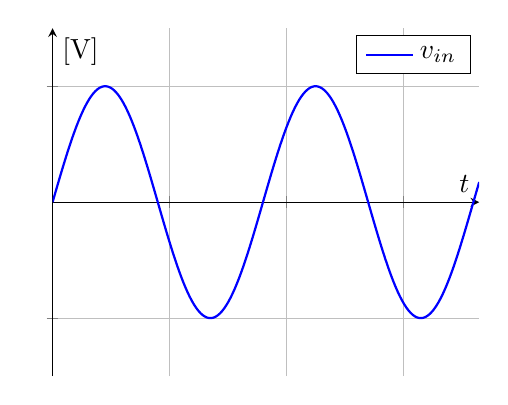
\begin{tikzpicture}
      \begin{axis}[
          axis lines=middle,
          xlabel={$t$},
          ylabel={[V]},
          xticklabels={},
          yticklabels={},
          domain=0:730,
          samples=200,
          grid=both,
          width=7cm,
          height=6cm,
          ymin=-3, ymax=3,
          xmin=0, xmax=730,
        ]
        \addplot[blue, thick] {2*sin(x)};
        \addlegendentry{$v_{in}$}
      \end{axis}
    \end{tikzpicture}
  \end{minipage}
  \begin{minipage}[t][5cm][c]{0.5 \textwidth}
    \centering
    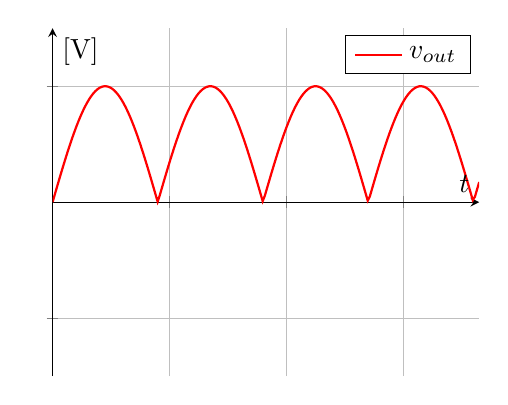
\begin{tikzpicture}
      \begin{axis}[
          axis lines=middle,
          xlabel={$t$},
          xticklabels={},
          yticklabels={},
          ylabel={[V]},
          domain=0:730,
          samples=200,
          grid=both,
          width=7cm,
          height=6cm,
          ymin=-3, ymax=3,
          xmin=0, xmax=730,
        ]
        \addplot[red, thick] {abs(2*sin(x))};
        \addlegendentry{$v_{out}$}
      \end{axis}
    \end{tikzpicture}
  \end{minipage}
  \caption{señales de entrada y salida}
\end{figure}

Para comprender su funcionamiento, podemos analizar por separado el comportamiento del circuito durante el semiciclo positivo y el
semiciclo negativo, considerando que hay una carga conectada.

Durante el semiciclo positivo, el terminal superior de la entrada presenta un mayor potencial que el inferior. En esta condición, los diodos
D2 y D3 se encuentran polarizados en directa, mientras que D1 y D4 están polarizados en inversa. La corriente fluye desde el terminal
superior, atravesando el diodo D2, pasando por la carga, luego por el diodo D3, y finalmente hacia el terminal inferior de la entrada.

Durante el semiciclo negativo, el terminal inferior de la entrada se encuentra a mayor potencial que el superior. En este caso, los diodos
D1 y D4 quedan polarizados en directa, y D2 y D3 en inversa. La corriente fluye desde el terminal inferior, pasando por el diodo D4,
atravesando la carga en el mismo sentido que en el semiciclo positivo, y continuando por el diodo D1 hasta llegar al terminal superior.

Como resultado, en ambos semiciclos la corriente atraviesa la carga en la misma dirección, lo que permite obtener una señal rectificada
de onda completa.

\begin{figure}[h]
  \begin{minipage}[t][8cm][c]{0.5 \textwidth}
    \centering
    \begin{circuitikz} [circuitikz/diodes/scale=0.7, american]
      \draw (0,0) coordinate(top bridge) to [full diode, *-*, l={\footnotesize D2}, f={i}] ++(2,-2) coordinate(right bridge)
      to [full diode, *-*, invert, l={\footnotesize D4}] ++(-2,-2) coordinate (bottom bridge)
      to [full diode, *-*, invert, l={\footnotesize D3}, f_<=i ] ++(-2,2) coordinate (left bridge)
      to [full diode, *-*, l={\footnotesize D1}] (0,0);

      \draw (top bridge) to[short, -o, f_<={i},] ++(-3.5,0) coordinate(inA);
      \draw (bottom bridge) to[short, -o, f=i] ++(-3.5,0) coordinate(inB);
      \draw (right bridge) to[short] ++(1,0) coordinate(outA);
      \draw (left bridge)to[short] ++(-0.3,0) to[short] ++(0,-3) to[short, f_<=i] ++(5.3,0) coordinate(outB);

      \draw (outA) to[R, v_=$v_L$, f=i] (outB);

      \node at ($(inA)!0.5!(inB)$) []{$v_{in}$};

      \node at ($(inA) +(-0.4,0)$) []{+};
      \node at ($(inB) +(-0.4,0)$) []{-};

    \end{circuitikz}
    \caption{Semiciclo positivo}
  \end{minipage}
  \begin{minipage}[t][8cm][c]{0.5 \textwidth}
    \centering
    \begin{circuitikz} [circuitikz/diodes/scale=0.7, american]
      \draw (0,0) coordinate(top bridge) to [full diode, *-*, l={\footnotesize D2}] ++(2,-2) coordinate(right bridge)
      to [full diode, *-*, invert, l={\footnotesize D4}, f<={i}] ++(-2,-2) coordinate (bottom bridge)
      to [full diode, *-*, invert, l={\footnotesize D3}] ++(-2,2) coordinate (left bridge)
      to [full diode, *-*, l={\footnotesize D1}, f>_={i}] (0,0);

      \draw (top bridge) to[short, -o, f_=i] ++(-3.5,0) coordinate(inA);
      \draw (bottom bridge) to[short, -o, f<=i] ++(-3.5,0) coordinate(inB);
      \draw (right bridge) to[short] ++(1,0) coordinate(outA);
      \draw (left bridge)to[short] ++(-0.3,0) to[short] ++(0,-3) to[short, f_<=i] ++(5.3,0) coordinate(outB);

      \draw (outA) to[R, v_=$v_L$, f = i] (outB);

      \node at ($(inA)!0.5!(inB)$) []{$v_{in}$};

      \node at ($(inA) +(-0.4,0)$) []{-};
      \node at ($(inB) +(-0.4,0)$) []{+};

    \end{circuitikz}
    \caption{Semiciclo negativo}
  \end{minipage}
\end{figure}

\subsection{Elección de los diodos}

Para dimensionar correctamente los diodos del puente, partimos de que la fuente debe entregar 1,5\,A continuos a la carga. Sin embargo, cada
par de diodos sólo conduce durante un semiciclo (50\,\% del tiempo), de modo que la \emph{corriente media} que atraviesa cada “rama” del
puente es:


\begin{equation}
I_{\mathrm{media\;por\;rama}} = 1{,}5\;\mathrm{A} \times 0{,}5 = 0{,}75\;\mathrm{A}.
\end{equation}

Si usásemos diodos de la serie 1N4001–1N4007 (1\,A de corriente continua), tendríamos un margen de sólo $0{,}25\A$ sobre esa
corriente media. Además, el regulador LM317, aunque nominalmente entrega 1,5\,A, puede generar picos de hasta 2,1\,A antes
de activar su protección interna, y esos picos también cruzan el puente de diodos.

Como los diodos de 2\,A no son habituales, elegimos la serie 1N5400–1N5408 (3\,A de corriente continua), que ofrece:

\begin{itemize}
    \item Suficiente margen sobre los 0,75\,A medios de cada rama.
    \item Capacidad de soportar picos transitorios sin acercarse a su límite máximo.
\end{itemize}

De este modo garantizamos un funcionamiento y seguro, minimizando el riesgo de sobrecalentamiento o daño por sobrecorriente.

\section{Filtro}
\label{sec:filtro}
La onda pulsante a la salida del rectificador no es apta para alimentar
equipos electrónicos por ello se le agrega un capacitor de filtro para
alizarla, la formula para calcular el mismo es:

\begin{equation}
  C=\frac{I_L}{2 \cdot f_{salida} \cdot \Delta V}
  \label{eq:filtro}
\end{equation}

formula extraida del libro Amplificadores Operacionales y Circuitos Integrados Lineales Coughlin-Driscol. Esta formula predice
muy bien el riple obtenido experimentalmente.
Siendo $\Delta V$ la tension pico a pico del ripple

En nuestro caso, utilizaremos un capacitor de $3300\uF$. Podemos calcular el valor esperado de $\Delta V$ despejando de \ref{eq:filtro}.

\begin{equation}
  \begin{aligned}
    \Delta V&=\frac{I_L}{2 \cdot f_{salida} \cdot C}\\
    \Delta V&=\frac{1{,}5\A}{2 \cdot 100\Hz \cdot 3300\uF}\\
    \Delta V&= 2{,}272 \V
  \end{aligned}
\end{equation}

\section{Regulador de circuito integrado}
La funciónes del regualdor son:

\begin{itemize}
  \item Mantener estable la tensión de salida de la fuente sin importar las variaciones tanto de la corriente de carga como de la red electrica.
  \item Reducir el ripple en un orden de mil veces.
\end{itemize}

En nuestra fuente, utilizaremos un LM317 en encapsulado TO-220.

\begin{figure}[h]
  \centering
  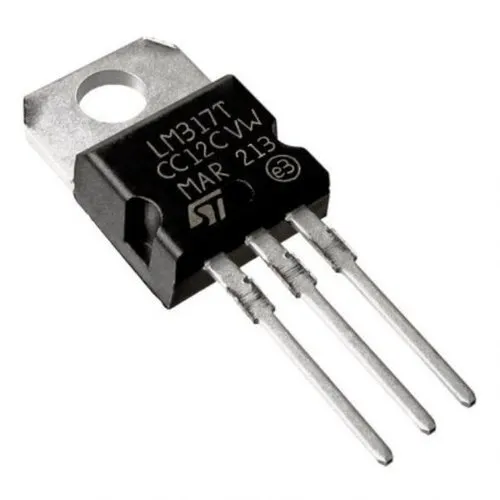
\includegraphics[width=0.35\textwidth]{images/LM317-TO220.png}
  \caption{LM317 encapsulado T0-220}
\end{figure}

El regulador cuenta con 3 terminales \textbf{IN}, \textbf{OUT} y \textbf{ADJ}.

Su principio de funcionamiento se basa en mantener una tensión constante de referencia $V_{ref} = 1.25\V$ entre la salida y el pin de ajuste, independientemente
de la tensión de entrada o de la carga conectada. Además, la corriente que circula por el pin ADJ, llamada $I_{adj} = 50 \uA$, también se mantiene constante.

\begin{figure}[h]
  \centering
  \begin{circuitikz}
    \ctikzset{resistors/scale=0.7}
    \draw  node[rectangle,draw, minimum width=3cm,minimum height=2cm, label={[below]north:LM317}, label={[right]west:IN},
      label={[above]south:ADJ}, label={[left]east:OUT}](LM317){}  ;
  
    \draw (LM317.west) to[short, -o] ++(-1,0) coordinate(inA);
    \draw (LM317.east) to[short, -*] ++(1.5,0) to[R=$R_1$, f>^=$I_{R_1}$] ++(0,-2.5) coordinate(nodo);
    \draw (LM317.south) to[short] ++(0,-1.5) to[short, -*, f=$I_{adj}$] (nodo) to[vR=$R_2$] ++(0,-1.5) coordinate(R2s) to[short, *-o] ++(-5.5,0) coordinate (inB);
    \draw (LM317.east) to[short, -o] ++(3.5,0) coordinate (outA);
    \draw (R2s) to[short, -o] ++(2,0) coordinate (outB);
    \draw (R2s) node[ground]{} ;

    \coordinate (p1) at ($(LM317.east)+(1,-0.2)$);
    \coordinate (p2) at ($(nodo)+(-0.5,0.2)$);
    \coordinate (p3) at ($(p1) !0.5! (p2)$);
    \draw [stealth-stealth] (p1) -- (p2);
    \node at ($(p3) +(-.5,0)$) []{$V_{Ref}$};

    \node at ($(inA) +(-0.4,0)$) []{+};
    \node at ($(inB) +(-0.4,0)$) []{-};
    \node at ($(outA) +(0.4,0)$) []{+};
    \node at ($(outB) +(0.4,0)$) []{-};

    \node at ($(outA)!0.5!(outB)$) []{$V_{out}$};
    \node at ($(inA)!0.5!(inB)$) []{$v_{in}$};

  \end{circuitikz}
  \caption{Regulador}
\end{figure}


Entendiendo esto, podemos deducir la ecuación de la tension de salida $V_{out}$.

\begin{equation}
  \begin{aligned}
    V_{out} &= V_{ref} + V_{R2}\\
    V_{out} &= V_{ref} + \left(I_{adj} + \frac{V_{ref}}{R_1}\right)R_2 \\
    V_{out} &= V_{ref} \left(1 + \frac{R_2}{R_1} \right) + I_{adj}  R_2 \\
  \end{aligned}
\end{equation}

Si tenemos en cuenta los valores $R_1=220\ohm$ y $R_2=0-5\kohm$ 

Podemos calcular los valores máximos y minimos de salida del regulador.

\begin{equation}
  \begin{aligned}
    V_{out MAX} &= 1{,}25\V \left(1 + \frac{0}{220\ohm} \right) + 50\uA \cdot 0 \\
    V_{out MIN} &= 1{,}25 \V \\
    V_{out MIN} &= 1{,}25\V \left(1 + \frac{5\kohm}{220\ohm} \right) + 50\uA \cdot 5\kohm \\
    V_{out MAX} &= 29{,}9 \V \\
  \end{aligned}
\end{equation}

Otros datos importantes obtenidos de la hoja de datos del fabricante son:

\begin{center}
  $I_{MAX}=1.5\A \quad V_{Diff-MAX}=V_{in}-V_{out}=40\V \quad T_{juntura-max}=125\Celsius \quad P=15\W$ 
\end{center}

Con estos datos podemos explicar la necesidad de poder alternar entre dos tensiones de transformador planteada
en la sección \ref{sec:transformador}.

En el caso de tener una $V_{in}=24\V$ y $V_{out}=1{,}25\V$ entregando una corriente de $I=1{,}5\A$ la potencia disipada
en el LM317 sería:

\begin{equation}
  \begin{aligned}
    P &= \left( V_{in} - V_{out}\right) I \\
    P &= \left( 24\V - 1{,}25\V\right) 1{,}5 \A \\
    P &= 34{,}125 \W
  \end{aligned}
\end{equation}

Lo que supera ampliamente la potencia maxima que puede disipar nuestro regulador.


\subsection{Protecciones internas}
  El regulador LM317 cuenta con diversas protecciones integradas que garantizan su funcionamiento seguro ante
  condiciones anómalas:

  \begin{itemize}
      \item \textbf{Protección contra sobrecorriente:} Cuando la corriente de salida supera el límite permitido, 
        el regulador activa un mecanismo de protección que evita daños internos.

      \item \textbf{Protección térmica:} Si la disipación de calor no es adecuada, debido por ejemplo a un 
        disipador insuficiente, la temperatura de la unión puede incrementarse más allá del valor seguro. En este caso, se activa una protección interna para evitar el sobrecalentamiento.

      \item \textbf{Límite de operación segura del transistor de salida:} Aunque no se supere el límite de 
        corriente, si existe una gran diferencia de potencial entre la entrada y la salida, puede ocurrir una 
        disipación de potencia que exceda la capacidad del regulador. En estas condiciones, también entra en 
        acción la protección interna.
  \end{itemize}
 
  \textbf{Nota:} En todos los casos anteriores, cuando se activa alguna protección interna, el regulador 
    interrumpe temporalmente su operación. Una vez que desaparece la condición que provocó la falla, el 
    dispositivo retoma su funcionamiento normal de forma automática.

\section{Fuente auxiliar}
  En algunos escenarios, es necesario que la fuente tenga como tension minima $0\V$ y no ese $1{,}25\V$, por lo
  que es necesario contrarrestar dicha tension de alguna forma. Por esto, se utilizará una fuente auxiliar
  que contrarreste estos $1{,}25\V$.
